\chapter{Eagle Eye}
\label{cha:eagle_eye}

% 30/40 pages

Eagle Eye is the product of this thesis and is our implementation of the requirements previously detailed. It is a visualization tool that enables the display and manipulation of a large image set at once. It is focused at the regular computer user that has a few thousand digital photographs stored on the computer. It allows navigation, through panning and zooming of the canvas where the image collection is disposed, sorting in different ways while also allowing filtering, either textual or visual.

In this chapter, we will go through how does Eagle Eye work, what are its components and how they interact.


\section{Overview}

Our requirements stated the need for features to be extracted from images, so we  started by creating a system to enable that. We then changed our focus to the visualization part of the work and redefined the general architecture of the work. The system is now composed of two main elements: the Backend, which is the system that extracts features from the images and prepares everything to be displayed; and the Visualization which performs the display from the images and their extracted features to the user.


This is the overview of the system that we will now detail in the following sections.




\hide{ %%%%%%%%%%%%%%%%%%%%%%%%%%%%%%%%%%%%%%%%%%%%%%%%%%%%%%%%%%%%%%%%%%%%%%%%%%%%%%%%%%%%%%


\section{Design Decisions} % (fold)
\label{sub:design_decisions}

\subsubsection{DeepZoom} % (fold)
\label{ssub:deepzoom}

After analyzing some visualization technologies that allowed easy display and manipulation of images \todo{Insert a bunch of ``useless'' tech}, Microsoft’s Silverlight, with its DeepZoom technology, proved to be the best choice.

DeepZoom enables the use of multiple resolution images for efficient display at various zoom levels and, for instance, is used for the display of gigapixel photos \footnote{Gigapixel photo of San Francisco: \url{http://theeyegame.com/DZSL/TwinPeaks5DMk2}}, where the user can view the whole image or zoom in the small details, or for collections of photos where the user can zoom between a view of multiple images and the details of a single image\footnote{Hard Rock Memorabilia: \url{http://memorabilia.hardrock.com}}. So far, usages of DeepZoom have been restricted to promotion websites, art galleries and other closed usages.

\red{This should be about the multi-scale images and not about DeepZoom $\rightarrow$ }Our work aims at bringing this technology to the regular user, in a much simpler and dynamic way.

Although DeepZoom seemed a great technology, it relies on Silverlight, which by itself isn't as good as using a full-fledged desktop application framework like \ac{WPF} or other frameworks native to their platforms. This created some undesired limitations like the need to have two separated parts of the system, the visualization and the backend, and other smaller problems like limited access to the disk from the visualization part.

To create a DeepZoom application, some pre-processing is required before hand to create multiple versions of each image in various resolutions and also to create imagery of a global view of the collection, also in multiple resolutions. This enables DeepZoom to only load the appropriate set of images for a certain zoom state, keeping the bandwidth (if used on the Internet) and memory requirements to a manageable level. This required pre-processing is done once on the backend. The visualization then uses the generated data to display the collection, being, at this point, totally independent from the original image files belonging to the user.

\subsubsection{Separation of Frontend and Backend}

As we just said, there's a need for previous processing to occur

% subsubsection deepzoom (end)
% subsection design_decisions (end)

} % end hide


\section{Backend} % (fold)
\label{sub:backend}

The backend is one of the two parts that make Eagle Eye. Its purpose is to extract information from images and set everything up for the Visualization.

Currently it is a command line utility that allows the user to enter paths for folders containing image files. The system will then read those images, gather their metadata, process them with the existing plugins to extract visual features and, finally, generate and output the multi-scale imagery \red{(ainda não se falou disto)} alongside with control metadata for the visualization.

We will now detail its architecture, and implemented feature extractors.

\subsection{Architecture of the Backend}

The Backend comprises a library manager to hold the images, feature extractors to process those images and persistence to save all generated data.

Figure \ref{fig:arch} is a simple explanation of the components. The Eagle Eye part is the main application, containing the library and feature extractor managers. Both deal with files on the disk, JPEG image files and DLL extractor plugins, respectively. The user interacts with the core of Eagle Eye which currently provides a command line interface for its actions, like the image import and plugin execution. The import gathers the files and their metadata, to be later accessed by the plugins for processing. Plugins store the resulting data inside the library manager and can be accessed afterwards for outputting by a special plugin.

We will now go through this components in more detail. 

\begin{figure}[ht]
	\centering
		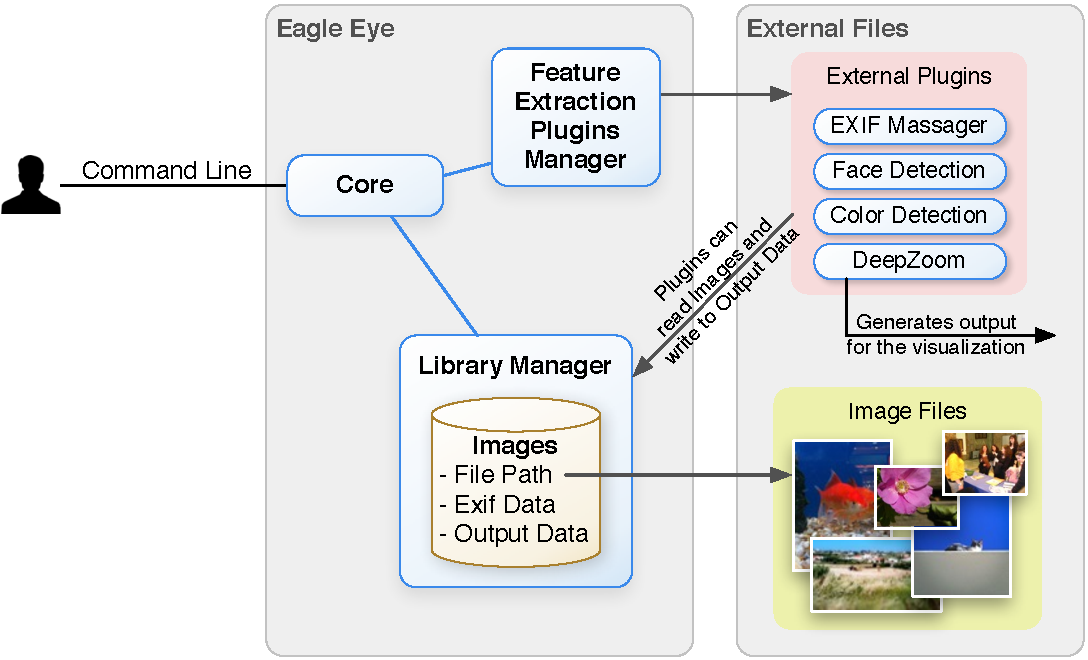
\includegraphics[scale=0.7]{Figures/Architecture_v2.pdf}
	\caption{Basic architecture of Eagle Eye's backend}
	\label{fig:arch}
\end{figure}


\subsubsection{Library Manager} % (fold)
\label{ssub:library_manager}

The system displays images and, therefore, it needs to know what to show. This is where the library manager comes in. It creates a database which indexes existing JPEG image files stored on the user's computer and makes this information available for other modules to use. It is designed to be used with digital photographs which contain the aforementioned EXIF metadata like time, date, camera information, or location. This information is gathered upon import and is available throughout the Backend.

We explored a few ways to develop the image import process and we rested at the fastest we found. The user refers a folder to be imported and we use a third-party program, ExifTool\footnote{ExifTool is a utility that allows easy read and write of file metadata. \url{http://www.sno.phy.queensu.ca/~phil/exiftool}}, to crawl through the user-specified folders while identifying all the JPEG images and returning their \ac{EXIF} metadata which is then stored by our system (\fig{arch:import}).

\begin{figure}[ht]
	\centering
		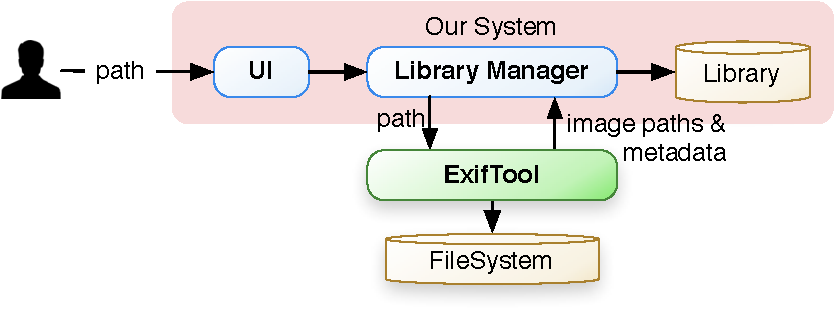
\includegraphics[scale=0.6]{Figures/import.pdf}
	\caption{Process in use by our system of importing a folder using ExifTool.}
	\label{fig:arch:import}
\end{figure}


Another option for importing metadata was to invoke ExifTool as part of a \ac{FEP}. Although that could fix a couple of problems with the current  implementation, it doesn’t make the metadata as ubiquitous as needed. Most \acp{FEP} rely on some \ac{EXIF} plugins to work correctly and the current implementation doesn’t easily allow inter-\ac{FEP} data-sharing.

% subsubsection library_manager (end)




\subsubsection{Feature Extraction} % (fold)
\label{ssub:FeatureExtraction}

To enable the Visualization to arrange the images on the screen in different ways, they need to be classified. Some information is easy to obtain and compare, like when the photograph was taken. Other information needs to be extracted, like the number of people in the photo or what are the most relevant colors in the image. \Fig{fe} is a short example of what feature extraction is all about.

\begin{figure}[ht]
	\centering
		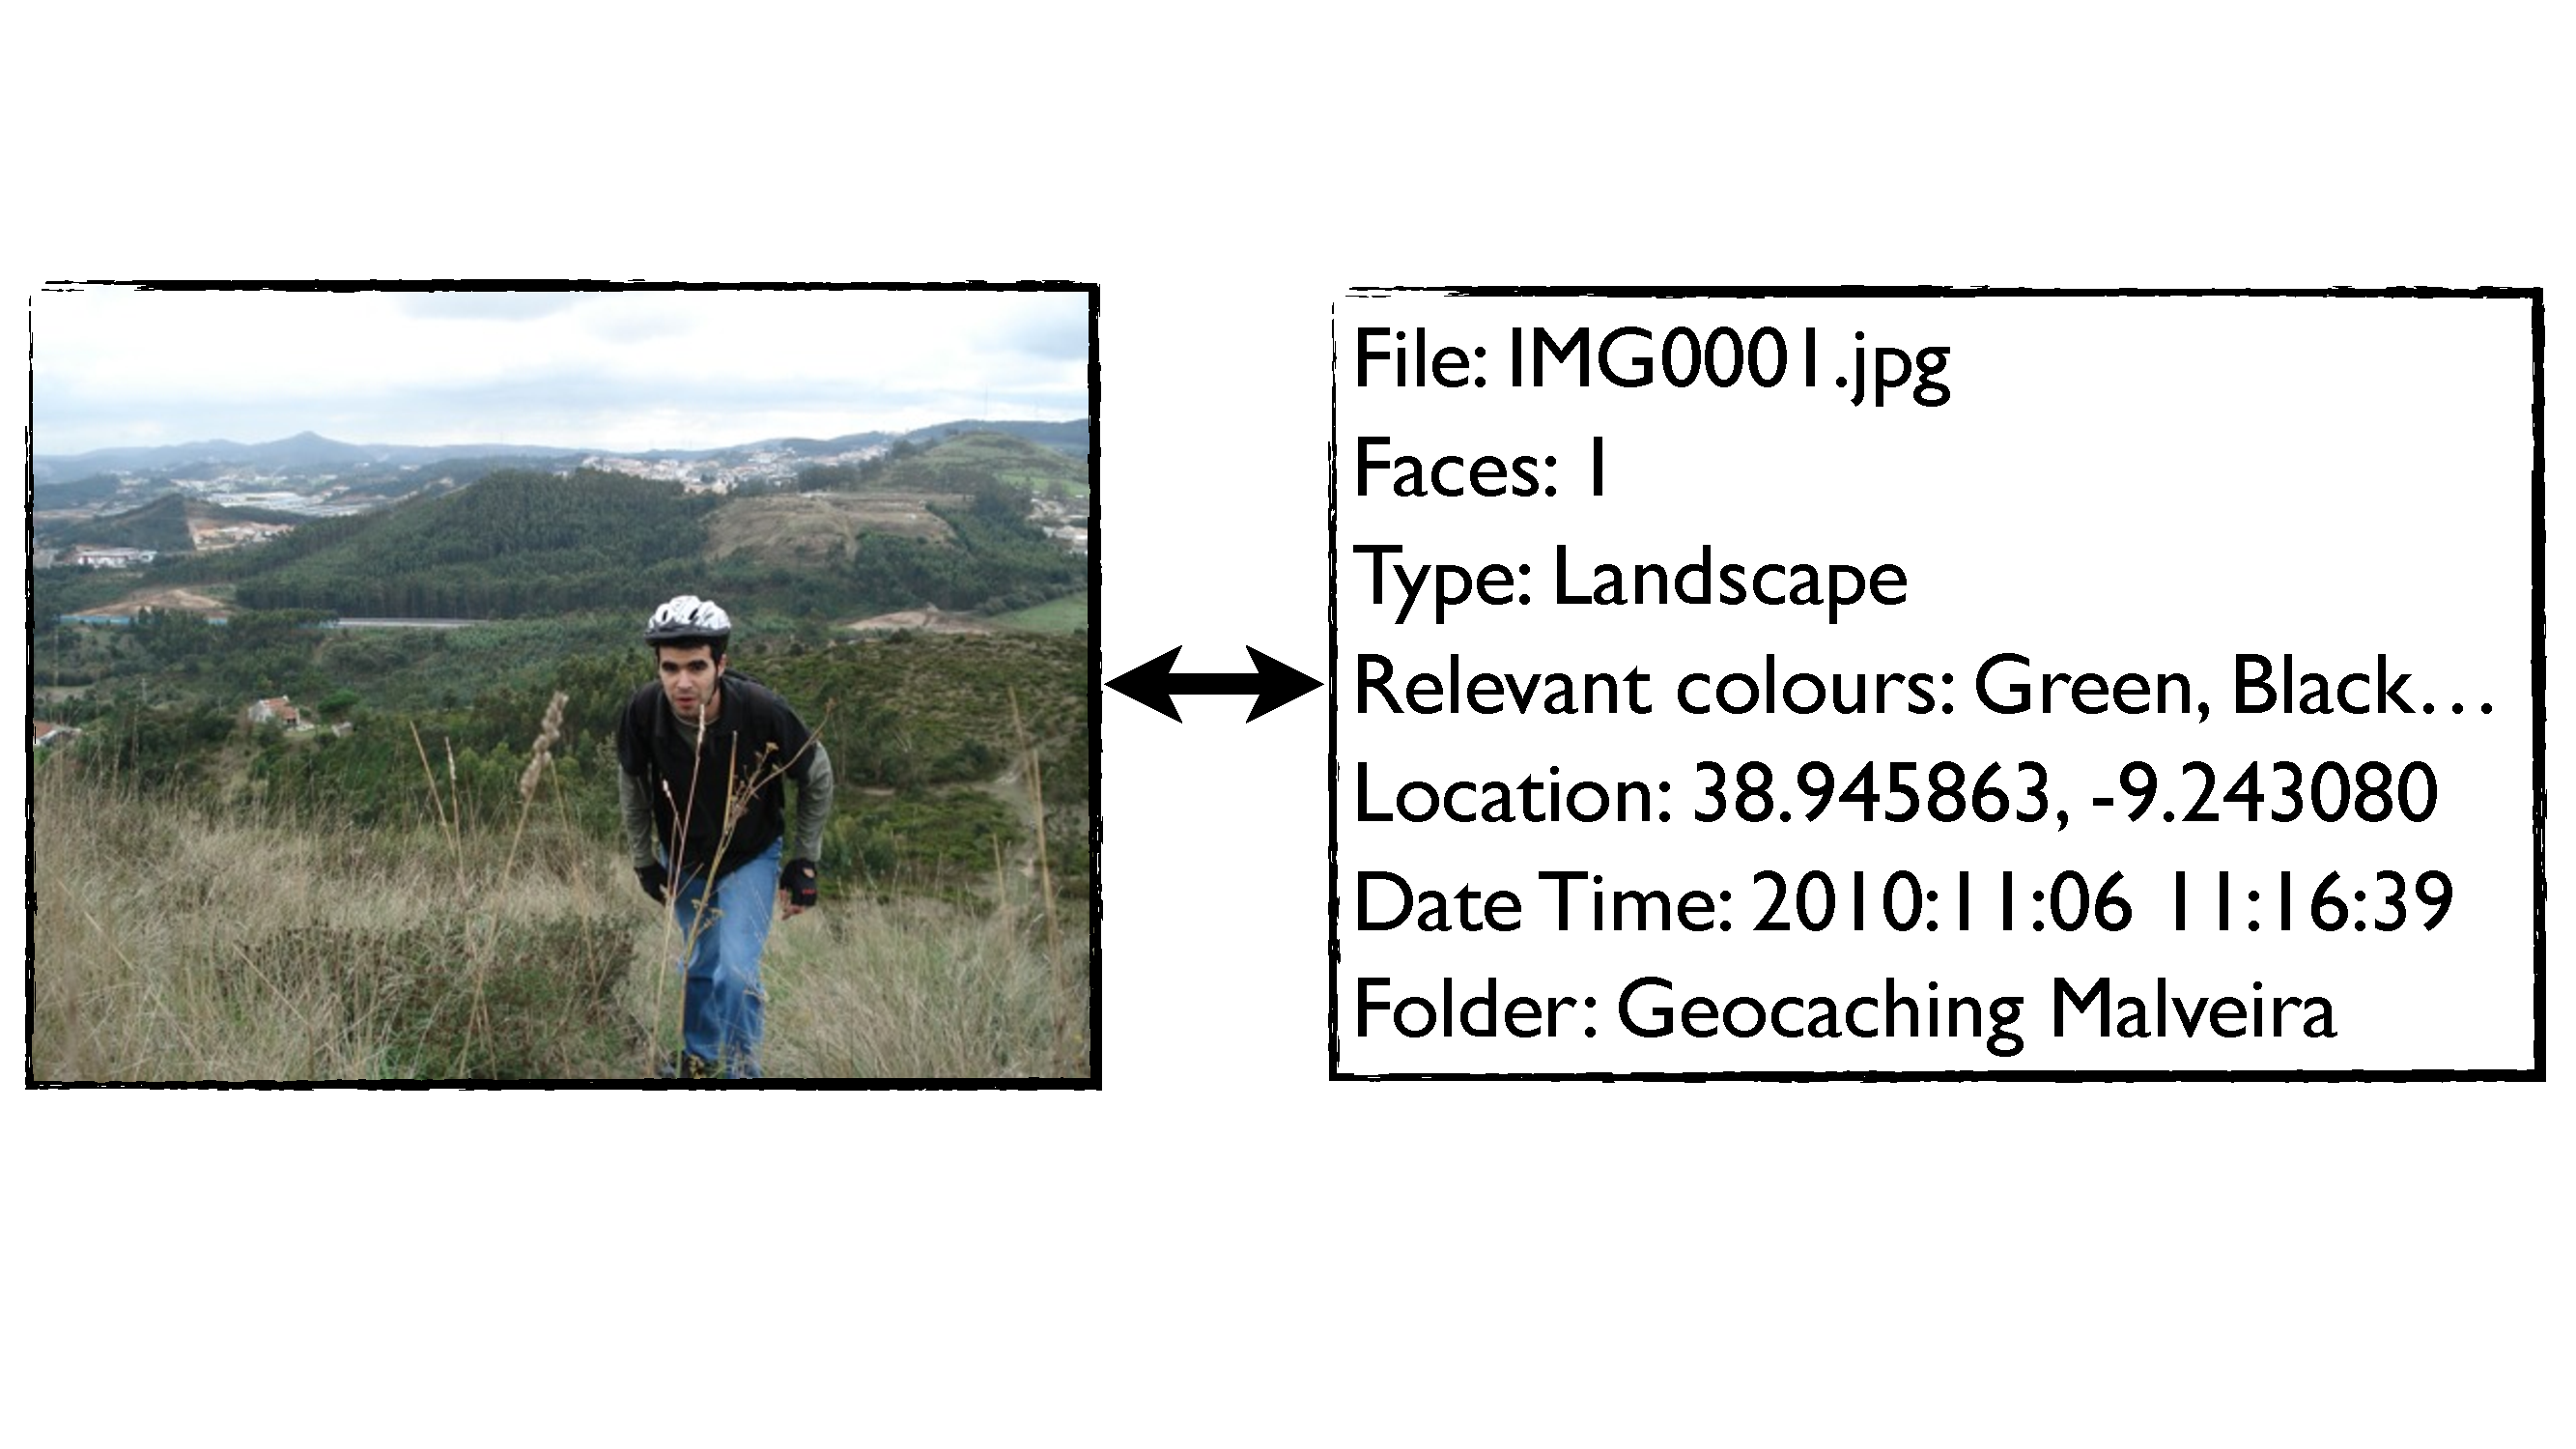
\includegraphics[width=0.72\columnwidth]{Figures/fe.pdf}
	\caption{Example of information extracted from an image.}
	\label{fig:fe}
\end{figure}

We had a few ideas for extracting features from images and, to be possible to add more along the way, we developed a plugin system to ease the creation of other feature extractors in the future.

Each Feature Extraction Plugin is separated from the main system. They need to implement a common interface and are given the ability to access the image data from the library, and save the computed data back. They have freedom to access the image file or its \ac{EXIF} information. They should, in the end, store the processed data in a specified way so it gets exported to the visualization. Implemented plugins will be explained in section \ref{sub:plugins}.

% subsubsection Feature Extraction (end)




\subsubsection{Persistence} % (fold)
\label{ssub:Persistence}

Persistence of both library and plugin data are required so the system doesn't lose information that took time to generate. To ease the interaction with a database system, we created a database abstraction layer that hides the complexities of interacting with said system. It also allows us to change to another database system if we see the need for it. We chose Oracle's Berkeley DB\footnote{Berkeley DB is a high-performace, embeddable, key-value, file-based database available at \url{http://www.oracle.com/technetwork/database/berkeleydb}} for its speed in retrieving data.

With this layer we can hide some optimization complexities like lazy-saving and lazy-loading. We use lazy-saving to save data to disk by chunks instead of doing it on each small update, speeding up the update process. Lazy-loading is not yet implemented but it is essential with libraries with tens of thousands of images, where keeping a complete library in memory is not feasible.

% subsubsection database_abstraction_layer (end)

%subsection arch backend (end)












\subsection{Feature Extraction Plugins} % (fold)
\label{sub:plugins}

Back in the Solution Requirements chapter (\ref{reqs:features}), we detailed some possible features that were interesting to be used in this work. In this section we will detail what extractors have been implemented.

Currently, we have four feature extraction plugins:
\begin{myitemize}
	\item Selection of useful image metadata
	\item Detection of image’s main color
	\item Face detection
	\item Generation of multi-scale imagery
\end{myitemize}

We now proceed to the explanation of each one of this plugins. 

\subsubsection{Selection of useful image metadata}

This plugin acts as a filter for all the available \ac{EXIF} tags. It picks the most relevant ones, codes them in a pre-defined way and appends them to the rest of the information to be exported for the visualization.

Information when the photo was captured, what device was used, the path where it resides or information about the location where the photo was taken are a good example of the most commonly relevant tags \todo{Ask users what other tags are relevant for them}. In the future, this set of extracted tags could be optionally set by the user.


\subsubsection{Detection of image’s main color}

Sometimes people don’t recall where or when a photo was taken, or where is it, but they vaguely remember that the photo had some dominant colors, like the red of a parrot in a green background (\fig{parrot}). This kind of information can be helpful when searching for a photo in a collection.

\begin{wrapfigure}{r}{0.3\textwidth}
	\vspace{-20pt}
	\begin{center}
		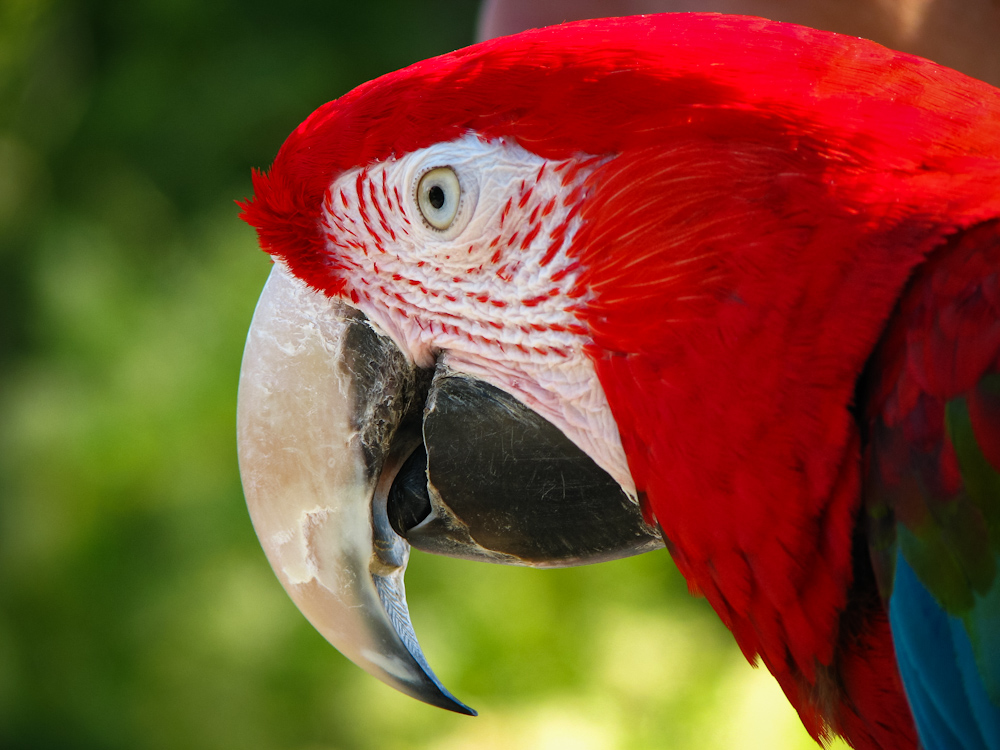
\includegraphics[width=0.29\textwidth]{Figures/parrot}
	\end{center}
	\vspace{-20pt}
	\caption{A colorful photo.}
	\vspace{-5pt}
	\label{fig:parrot}
\end{wrapfigure}

Color extraction from images has been a long standing problem \cite{Wan:2011bg,Strong:2009p413,Gabbouj:2009en,Girgensohn:2009:MOP:1502650.1502711,Zaheer:2010p3735,Datta:2008p1604,Chang:2007bt}. We wanted to extract the most perceptible colors from images so, in the parrot example (\fig{parrot}), the system should associate the image with the colors red, green, white and black and avoid colors that have little relevance, like the small blue of  the feathers and also ignore small tonal variances in the reds and greens.

For that we explored two methods that reduce the number of colors in an image to the most essential ones, the first being an adaptive method, selecting a few averaged colors from the image and the second using a palette as reference to select the colors.

A common JPEG photo can contain 16.8 million different colors. Our adaptive method reduces the possible colors to less than ten\footnote{We tried with multiple options from one color to ten colors and the results vary from image to image}. The obtained colors are chosen by averaging the colors in the image, so if there's a lot of blue tones, a single, averaged blue will be replacing those tones (see the middle image of \fig{sky}). In areas that have little tonal variation of the color, the resulting color will be very similar to the original (like in the right image of \fig{sky}). But sometimes this method fails to save important colors when they occupy a relatively small area of the image or if the image doesn't have a strong contrasts (shown by the left image in \fig{sky}).

\begin{figure}[ht]
	\centering
		\includegraphics[width=\columnwidth]{Figures/colorreduction.png}
	\caption{Three images where the left half is the original version and the right half is a version with very limited number of colors provided by the adaptive method.}
	\label{fig:sky}
\end{figure}




The second method uses a predefined color palette (\fig{colors}) which is an adapted mix between the eleven most recognizable colors (red, yellow, green, blue, purple, brown, orange, pink, black, white and grey)\footnote{Qiu \cite{Qiu:2007p1207} explains this are the most universal recognizable colors in any language.} and the 21 ColorAdd colors\footnote{ColorAdd is a 21 color catalog with symbols for each color designed specifically for color blind people. We used the colors as a reference, specially the light and dark variations.}. This mix has a great range of colors and each one can be easily named with recognizable words\footnote{We want to avoid names like ``Amaranth'' or ``Munsell'' that most people don't know about. A large list of this names can be found on \url{http://en.wikipedia.org/wiki/List_of_colors}.} which then could be assigned to the images. The images processed with this method get their colors changed to the most similar ones present in our palette. This assures that colors in a relatively small area or images with low contrast still get the deserved attention (\fig{pinkP}), unlike the adaptive method (\fig{pinkA}). This method doesn't reproduce the colors so well as the adaptive but, since we want to obtain generic colors, this one is more reliable.


\begin{figure}[!ht]
	\centering
		
\includegraphics[width=\columnwidth, height=45pt]{Figures/colours.pdf}
	\caption{Color palette in use for restricting the possible colors in an image.}
	\label{fig:colors}
\end{figure}


\begin{figure}[!htb]
  \begin{subfigmatrix}{3}
    \subfigure[Original image] {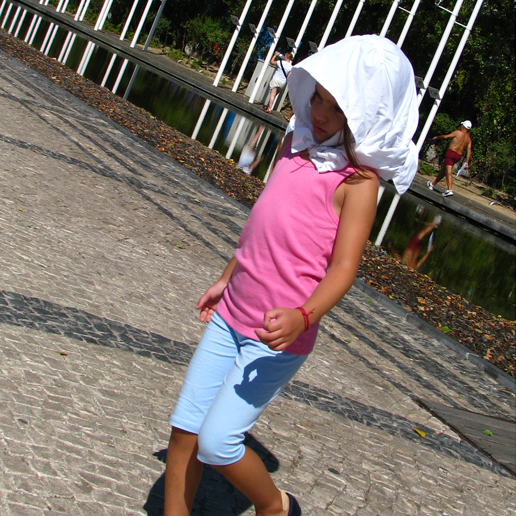
\includegraphics[width=0.328\linewidth]{Figures/pink1.png}\label{fig:pinkO}}
    \subfigure[Adaptive method]{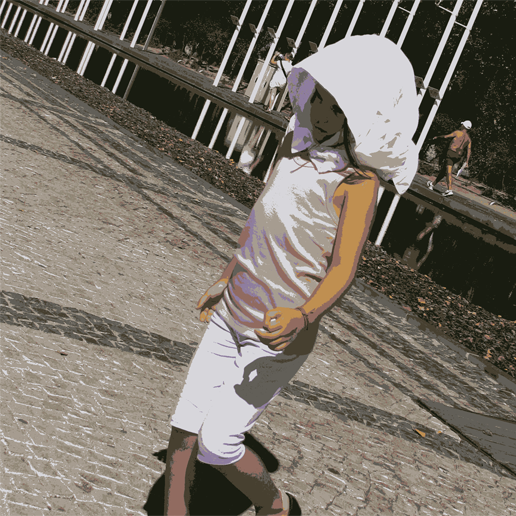
\includegraphics[width=0.328\linewidth]{Figures/pink2.png}\label{fig:pinkA}}
    \subfigure[Mapping method] {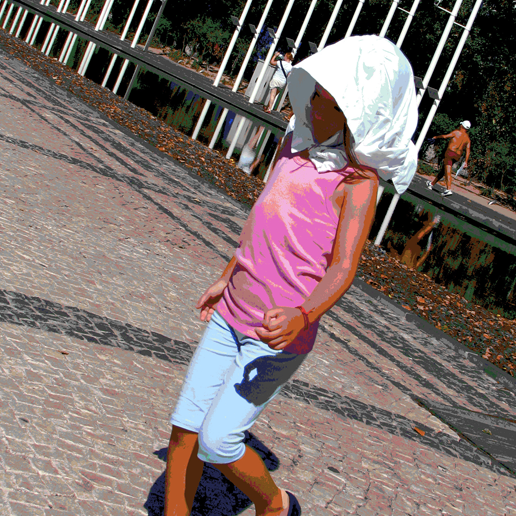
\includegraphics[width=0.328\linewidth]{Figures/pink3.png}\label{fig:pinkP}}
  \end{subfigmatrix}
  \caption{Comparison between the original image, the adaptive color reduction method failing to keep the pink and the blue colors and the color mapping method.}
  \label{fig:pink}
\end{figure}


This was the research we made to extract perceptible colors from images. We generated the above demonstration images using ImageMagick\footnote{ImageMagick is a software suite to create, edit, compose, or convert bitmap images. \url{http://www.imagemagick.org}} and its ``colors'' feature for the adaptive method and the ``remap'' for the palette method. Unfortunately, time was not on our side and we had to move to a simpler system. 

The current color extractor plugin does a simpler job of calculating the median color of the image and use the hue to index images.

We took some ideas from the work of Qiu et al\cite{Qiu:2007p1207} of exploring a method of image indexing that is fast and simple. On this work, images are sorted into ``bins'' according the their average color. This bins are divisions of color planes, indexed using binary trees allowing for very fast searches.

We used the open source library AForge.Imaging\footnote{AForge is a framework designed for developers and researchers in the fields of Computer Vision and Artificial Intelligence \url{http://www.aforgenet.com/framework/}} to obtain histograms for the images and compute their average color in RGB\footnote{Color model composed by red, green and blue \url{http://en.wikipedia.org/wiki/RGB}} and HSL\footnote{Color model composed of hue, saturation and luminance \url{http://en.wikipedia.org/wiki/HSL_and_HSV}} values. Both those values are then stored on the plugin-extracted data for each image. The images will be distributed into bins on the Visualization. We could assign bins at this point but, by not doing so, we are giving freedom to the users to change the number of bins used for display. We will discuss this on the Visualization sections ahead.


Although we didn't implement this plugin the way we desired, it demonstrates that color extraction is feasible and, with more time, a better method that does more than just averaging the colors, including detecting the most relevant ones, could be implemented.

\todo{show of differences between having the image reduced or not. something I never tested :P}




\subsubsection{Face Detection} % (fold)
\label{ssub:face_detection}

The face detection plugin is based on the open-source OpenCV library\footnote{OpenCV (Open Source Computer Vision) is a library of programming functions for real time computer vision. Available at \url{http://opencv.willowgarage.com}} which processes every image file and detects existing faces (\fig{faces1}).
 
\begin{figure}[ht]
	\centering
		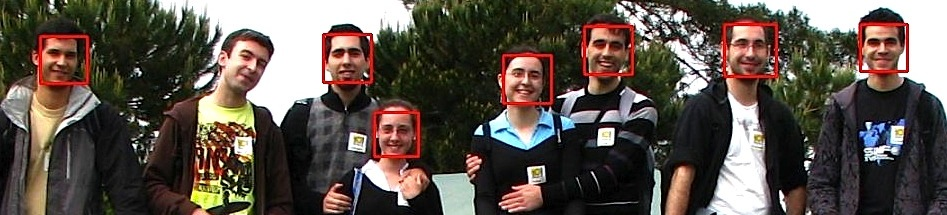
\includegraphics[width=\columnwidth]{Figures/faces1.jpg}
	\caption{Example of the OpenCV library detecting faces on a common photo.}
	\label{fig:faces1}
\end{figure}

No face recognition software is perfect. Usually if the software can detect every face, it will probably detect some other things in images that aren't faces (false positives). If it’s successful in only detecting faces, it will probably miss some other faces that aren't ideally positioned (false negatives). OpenCV is included in the latter, only detecting faces but also missing some that are tilted (like in \fig{faces1}) or turned on the side.


This process is quite computationally expensive and therefore we resize all the images down to a more acceptable size, making the process more than five times faster.

We tested 29 images, from six different cameras, ranging from one to ten megapixels, and containing up to thirteen faces. The test consisted in running face detection on each image, in its original size and in various resolutions from 2000 to 200 pixels on its longer side, comparing the number of faces recognised and the time needed to process them. The results can be seen in \fig{fdres}.

\begin{figure}[ht]
	\centering
		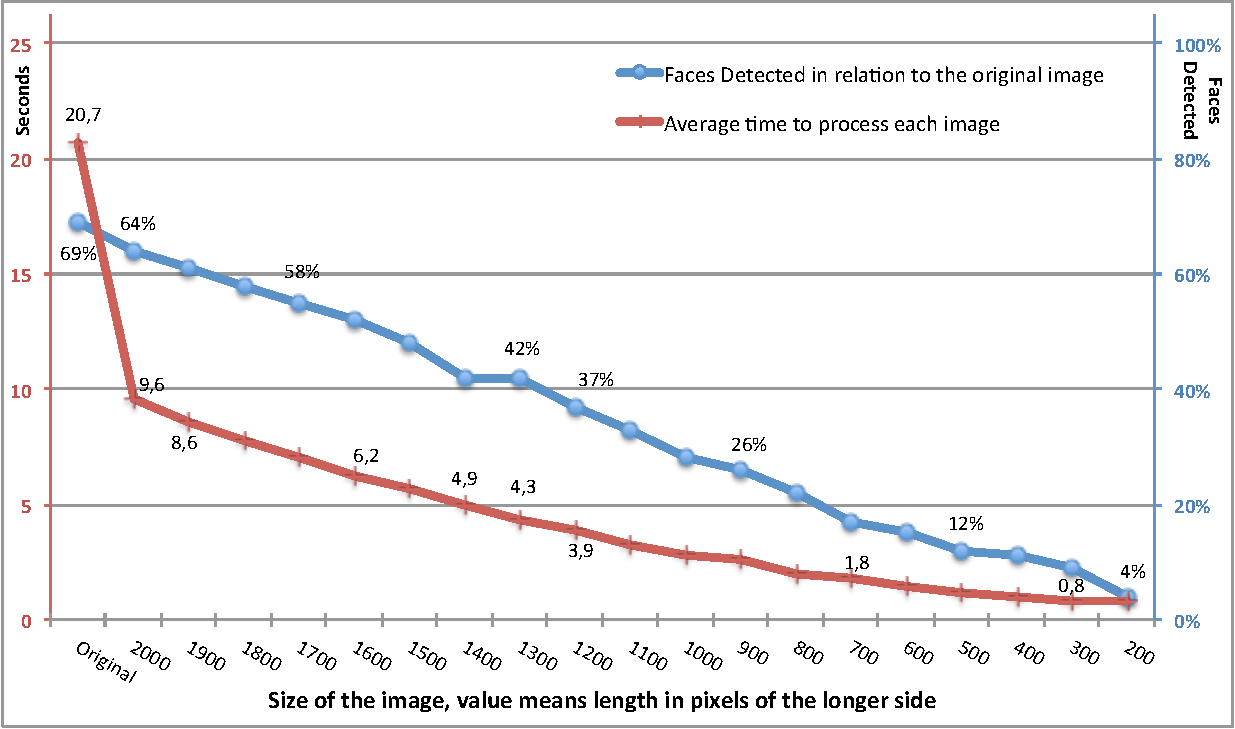
\includegraphics[width=\columnwidth]{Figures/graph2.pdf}
	\caption{Results of the face detection test. 100\% of faces is the actual faces present in the test images.}
	\label{fig:fdres}
\end{figure}

The purpose of this test is to identify how much can we reduce the images while maintaining a high recognition rate, we are comparing the recognition results of the downscaled versions to the original size and analyze the speedups and failures in recognition. We do include the number of faces actually present in the photos for comparison, corresponding to the 100\% value in \fig{fdres}.

We can see that by only reducing the images to 2000 pixels on the longer side, the processing time fell to less than half (20.7 to 9.6) without much loss in recognition (69\% to 64\%). The 1300 pixels was the chosen value for being the last with more than 40\% recognition rate (60\% of the full size image) and being 4.8 times faster\footnote{4.3 seconds per image versus 20.7; one hour and 10 minutes per thousand images versus almost six hours} than using the original image. In the future, with more tests, we can fine tune the resizing algorithm to get better results.



\hide{ver que caras falham primeiro para perceber o que aconteceu. As caras que se perdem são relevantes?}
% subsubsection face_detection (end)


\subsubsection{Generation of multi-scale imagery}

This plugin generates all the data files needed for the visualization to work. As referred previously, the visualization relies on the DeepZoom technology and it needs to process the images before they can be displayed. This plugin does exactly that.


Using a library from Microsoft, the plugin generates, for each image, a metadata file and a set of image files representing the original one at multiple scales, from a single pixel to a large, detailed image.

After passing through all images, the collection as a whole is subject of additional computation, this time generating imagery for all images as a single set and a metadata file that agglomerates all image sets used. This metadata file for the collection (called collection.xml) is then altered by the plugin to attach to each image, the data previously generated by the other plugins.

% subsection plugins (end)



%!TEX root = /Users/carlos/Dropbox/Thesis/Thesis.tex
\section{Visualization} % (fold)
\label{sub:visualization}

The greatest challenge of this work was the creation of the visualization part for its requirements. We will now describe this part of Eagle Eye, its architecture, visualization techniques, sorting and filtering capabilities.

\subsection{Overview}
We wanted to make the visualization simple and easy to use, while keeping it flexible enough to allow for an enjoyable experience.

After the backend has finished the all the processing that is needed, the visualization can be opened and all images that were added to the backend's processing list will appear. After loading the metadata, the user is presented with a set of options on the top toolbar, which is the only \ac{UI} needed to use the system. \todo{Add picture}

According to \todo{insert the reference of the dude who claimed that a 32x32px image was the minimum for recognition}, an image with 32 pixels per side is the minimum size that allows a user to recognize an image.

\red{Unsure about how well this fits here…} Upon loading Eagle Eye's visualization system, thousands of images might be displayed and this 32 pixel might not be met and, therefore, it might be difficult for the user to recognize what is on display from a single image, but since a lot of them are being displayed, the user might be capable of making sense of the groups by their main colors.

\subsubsection{The Canvas}

The canvas is the most relevant part of the visualization as it dynamically displays all the images previously selected by the user, at the same time. This may make the images barely recognizable and, therefore, the user has the possibility of manipulating the canvas to see and enjoy the images.
This means that the user can, at any time, use the mouse to drag the canvas around or, by clicking or scrolling, zoom in and out of the canvas. Zooming goes from the default view of thousands of images at the same time, until the full screen view of one of them, and everything in between in a smooth way.

\subsubsection{The toolbar}

The user can then use the functions on the toolbar to filter and sort differently. The toolbar is divided in three sections: Navigation, Display and Filtering.

The navigation section contains some basic functions that work similarly to the current web browsers. There are buttons for back and forward between display states and a save button for bookmarking the current display state, allowing the user to easily get back to it later.

The middle section contains two options to change the image display:  the sorting options and the display overlays button. The former presents the available sorting options for the current collection, based on the available metadata and on the best ways to display them. One of the options is selected at all times and the content is presented accordingly. Changing the selected option causes the images in display to move around to the new position and form a different sort order. This sorting and disposition options will be explained in a later section.
The other button in the display section of the toolbar enables or disables a layer of information on top of the images. This layer distinguishes the groups of images in display by painting them with a different colors and presents a name for them, depending on the selection sort option. Grouping will also be explained bellow. 

The third and final section of the toolbar is the filter section. It contains controls to filter images by using simple text and to visually select images on the canvas. This options will also be explained bellow.

\subsection{Disposition of Images on Canvas}
\label{sub:dispositions}

The different ways to dispose the images on the canvas was a matter that required some exploration of possibilities \refs. We chose a few options to allow some flexibility for the user, while trying to keep the interface simple.

We are now going to explain how do we sort images into groups and the different ways the user can arrange those groups on the canvas.

\subsubsection{Sorting images into groups}

As we've seen, the backend outputs metadata for each image. This metadata is loaded into the visualization application of Eagle Eye and is indexed by their type.

For instance, each image has an associated creation timestamp which will be aggregated by days, generating an image group for each day.

Similarly, the mean color associated with each image is indexed and groups are generated by dividing the hue spectrum in bins \todo{specify which and add the spectrum image}.

Another option is the grouping by device name, which usually allows to distinguish between who took the pictures if, for instance, different people have different cameras on the same event.

The last option currently available to the user is grouping by path which groups together the images that were already grouped by the user, on the file system. This allows for the display of an organization that is recognizable to the user, which can make a good starting point.

On the canvas, group boundaries are identifiable by discrete gray borders and, when the Show Overlays function is active, by color rectangles that also contain the groups' names.


\subsubsection{Different dispositions}

After having the images grouped by any of the sorting options referred on the previous section, the system has to know how to display them on the canvas.

We looked into various options \refs and picked the ones that we thought that made sense and also that would be easier for the user to understand. We chose a tree map view and a column-based linear view. Both of these are grid-based layouts, meaning that images are positioned inside a defined grid on the canvas. We also looked into free positioning systems like \refs but they make it harder for the user to understand the images within, since some images will be covered by others. When displaying thousands of images, it's important to make them easy to see, and mixing them up wasn't the appropriate thing to do. We focused on other ways for making it easier to the user see what matters and we will talk about them later on.

The first layout technique we employed was the tree map. The problem with tree maps is that they are designed for areas that can take many forms, from squares to thin lines \todo{insert tree map image}. Applying tree maps to images calls for the adaptation of the algorithms to make sure the areas can correctly hold the images and that all images in all groups have the same size and are positioned in the same grid, to make them easier to view. This ideas are supported by \todo{gajo} on his work in the Quantum treemaps. We tried to apply Quantum tree maps as our tree map algorithm but due to it's complexity and recurring problems, we adapted the tree maps of \todo{gajo}, as used in Prefuse \todo{verify} \refs to the reality of the image grid. This new algorithm was much easier to understand and implement, although  it might require a small fine running for a couple of edge cases.

Our tree map algorithm displays larger groups first, leaving the smaller ones to the end and makes an effort to layout groups as rectangles with an aspect ratio as close as possible to the screen's aspect ratio, for when the user zooms in, the groups fill the screen. There's also an effort to fill the space left between larger groups, making the display more compact and with less holes.

One problem of the tree map display is that group sequence is irrelevant. Groups are positioned by their size, which is unacceptable for sorting options that require some sequence, like sorting by time. For this we created a linear display that uses columns and displays groups sequentially. Each group may fill part of a column or various columns, depending on their size. With the aim of reducing wasted space, groups that fit on the wasted space left by the previous group use that space to display themselves. This is useful  to collapse the couple pictures the user might take of his regular day between days that he went on a trip and took a much larger number of photographs.

Currently we are using this layout system only for the date display since the use of columns makes visualization harder, requiring either some panning around the canvas or selecting the group using the filter tools explained ahead. This is an area we must improve, and we will discuss some ideas later on.


\subsubsection{Filtering} % (fold)

In addition to the sorting options explained above, Eagle Eye also provides the user with the ability to filter images. This allows the user to focus on a specific group of pictures that are his focus of interest at the moment.

For instance, the user might want to only see photos of a day, or a person, or person in a specific day or even pictures that are mostly blue.

For all this, Eagle Eye provides two ways to specify this kinds of constraints: using the filter bar or selecting pictures on the canvas, and we will now look into both them.

The filter bar's purpose mimics a regular search box, similar to the ones that exist on applications like Internet browsers, file browsers or photo browsers \refs: it provides a way for the user to type what he is looking for and get some suggestions to help him with the search. Since we wanted a simple \ac{UI}, we figured that we had to provide smart suggestions to the user, so that he can feel comfortable using it for multiple types of searches. Searches are performed immediately upon selecting the desired filter. Currently, searches are intersections (commonly ``and'') of the entries in the filter bar but after adding adequate \ac{UI}, it will be possible to also use unions (commonly ``or'').

Every piece of the metadata can be used as a filter and the suggestions list shows what are the available options and what type of metadata they relate to, for instance, when looking for a person's name, the ``keyword'' metadata type is shown, when searching for a place, both ``keyword'' and ``path'' types might be presented, if the path to the pictures included the place where they were taken.

This examples are quite simple but we wanted to go further and allow searches like ``Summer'', for all photos taken around the summer time in all years, ``May 2010'', for all pictures taken during that month, ``Has 2 people'' for photos that have been detected to have people in them. \red{Although some of these have not been implemented yet, they are in the plans.}

The second filter method allows the manual selection of images from the canvas, either by a common mouse drag-and-drop on the canvas or by selecting entire groups with a mouse click. This two interaction options can be activated on the respective button on the end of the toolbar \todo{image}. 

As explained above, the filter bar intersects its elements immediately after being added but that behavior in the function would make it impossible for the user to make multiple selections. So we made this feature allow various selections and only when the user forces the filtering that all the selections are unified and added to the rest of the intercession filters.

\red{Since the selections are displayed in the same way text filters are, the removal of a selection is made in the same way.}



\subsection{Architecture}

We will now take a look into the architecture of the visualization part of Eagle Eye.

\subsubsection{Metadata indexing}

At the center of the visualization is the DeepZoom canvas. By default, it displays images in the order they are specified on the ``collection.xml'' file, the file generated by the backend that identifies the multi-resolution imagery and images' metadata.

The ``collection.xml'' also contains some metadata for each image, added by the backend. The visualization parses the file and extracts this metadata which is then processed and indexed.

Since the transport is a text file, we used a simple, text based, key/value capable encoding \red{system}: JSON \refs. The backend encodes key/value pairs of metadata for each image \todo{meter um exemplo em código} and the visualization decodes and aggregates them in indexers, one indexer for each type of metadata. Eagle Eye has a few indexers that know how to read and process different types of data:
\begin{myitemize}
	\item{a generic indexer, for basic text or number values}
	\item{a date indexer, that gathers images by day}
	\item{a color indexer that gathers images by color, using \red{N} bins for \todo{lalala}}
	\item{a keyword indexer that indexes images by each one of the associated keywords}
	\item{a path indexer that indexes images by the folder where they resided when added}
\end{myitemize}

The indexers are managed by a metadata collection manager that handles, for instance, the XML parsing and creation and retrieval of indexers.

This indexers are the base for the sorting and disposition techniques we've covered on \ref{sub:dispositions}. Each indexer has attached the preferred way to be displayed, for instance, the path indexer works better when displayed using a tree map and thats what the ``Path'' button on the toolbar will use to dispose the images, but the date has two buttons, ``Date'' and ``Date (linear)'' because it makes sense for it to be displayed using both disposition techniques. \red{could be better}




\subsubsection{Canvas}

The canvas is the most important part of this work. Its core is from the DeepZoom framework and we use it to display lots of images in certain positions, according to the state of many variables. To hold all those options together and to help developing some more, we have created a state manager for the canvas.

A new canvas state object is created for each different set of options for the canvas. The object stores the options and computes the positioning of all images by picking those that have passed the filter, get the respective groups from the selected indexer, dispose them using the selected disposition algorithm and finally computing and saving the position for each image.

We use memoization to avoid repeated calculations for common display types. If a certain display has already been calculated, it will reuse the information on the saved state object to rearrange the canvas without going through the position calculations, allowing a faster interaction.


\subsubsection{Reducing Clutter}
\label{ss:stacks}

This work displays a great quantity of images at the same time and we thought that we could help the user by reducing some unnecessary clutter.

Sometimes users take more than one photo of the same thing and they do it for different reasons, some of them simple and others more technical. Some people just didn't like the previous photo or they want to make sure they have a few options to pick the best one and so they take more. Bursts of photographs are a similar case of this behavior but resulting in a larger image count.

Some more advanced photographic techniques require that the user takes more than one shot of something for merging in post processing. Examples of this techniques are panoramas, where a sequence of shots are merged to create a bigger image that what the camera lens is capable of, exposure bracketing, to overcome partial under or overexposure or focus bracketing, to increase the are of the image that is correctly focused.

Various shots of the same subject are generated by all of this motives and they clutter any image browser since they end up being multiple copies the same thing.

To help the user abstract himself from this similar images, we decided to come up with a way to collect them. Hsu et al. \cite{Hsu:2009p2696} used the idea of image grouping but probably not with a great implementation since it can be hard to see what is in the groups when they are collapsed and grouping was done manually. We chose a different path.

For our implementation, we decided to group images automatically based on the proximity of their capture timestamps, so every two images that were taken in a time span less then $t$ seconds are grouped together. After some experiments we decided on $t=4$ seconds which is more than enough for sequences of images that were taken automatically, gives some margin for manually taking another photo of the same thing, but is short enough for a regular user to take a picture, look at something else move the camera and take a picture of that.

For the display we decided to show all images of the group in the space of one, but displaying the first image at regular size and reducing the others to a smaller size, perceptible when looking closer and keeping the ability to zoom in on each of them and see them in fullscreen. This way we can reduce the clutter without fully hiding repeated images. \todo{images}

Obviously that this can have both false positives or false negatives but in our tests those were in a small number. \ac{UI} to fix that could be added but we don't feel that was essential.


%%%% Conclusion %%%%
\red{should make a section just for the chapter conclusion?}

To conclude this chapter, where we've seen what this work does and how it does it, we would like to add that many features and improvements could be added for an even better experience, but time and the focus of this work didn't allow us to do it. Even so, the Future Work (\ref{sec:futurework}) contains many ideas we have had which could bring this work to be a real world application.

% subsection visualization (end)




%%%% Conclusion %%%%
%\subsection*{Conclusion}

\vspace{2 em}


To conclude this chapter, where we've seen what this work does and how it does it, we would like to add that many features and improvements could be added for an even better experience, but time and the focus of this work didn't allow us to do it. Even so, the section on Future Work (\ref{future_work}) contains many ideas we had which could bring this work closer to a real world application.

% subsection visualization (end)





